\section{Research questions}
The research questions for the research project reported in this thesis was given in section 2.2 at page 6 as follows:
\begin{itemize}
	\item \textbf{RQ1:} Based on clinical guidelines, how can we define and represent a generic data structure that can be used to implement applications such as online guidelines or training games for such guidelines, and where applications can adapt to the level of their users?
	\item \textbf{RQ2:} Can the generic data structure in RQ1 be used to generate a specific data model for another domain such as paediatric asthma?
	\item \textbf{RQ3:} How can we use the data model in RQ2 to implement a game for guideline training that can adapt to the level and progression  of users?
	\item \textbf{RQ4:} Is the guideline meta model at an abstraction level such that it can be used for other guidelines? 
\end{itemize}
\section{Evaluations}
\subsection{Evaluation of the models}
To evaluate our model, we have decided to model the paediatric pneumonia guideline \parencite{RepublicofKeny2016}. As we have a strict time limitation it is better for us to evaluate a respiratory condition, as we have already worked with a respiratory condition in asthma. There is quite a lot of work for software developers to learn a new clinical guideline, so we save a lot of time when the concepts are similar.

In figure \ref{fig:PneumoniaEntityGraphExcerpt} we have modelled the excerpt of the entity model of the paediatric pneumonia guideline \parencite{RepublicofKeny2016}. We have removed unnecessary vertices such as Investigation and Surgery, as neither the pneumonia guideline nor the possible asthma guideline use them. On the Diagnosis vertex we now have a new inheritance. We'll soon explain.

\begin{figure}[h!]
	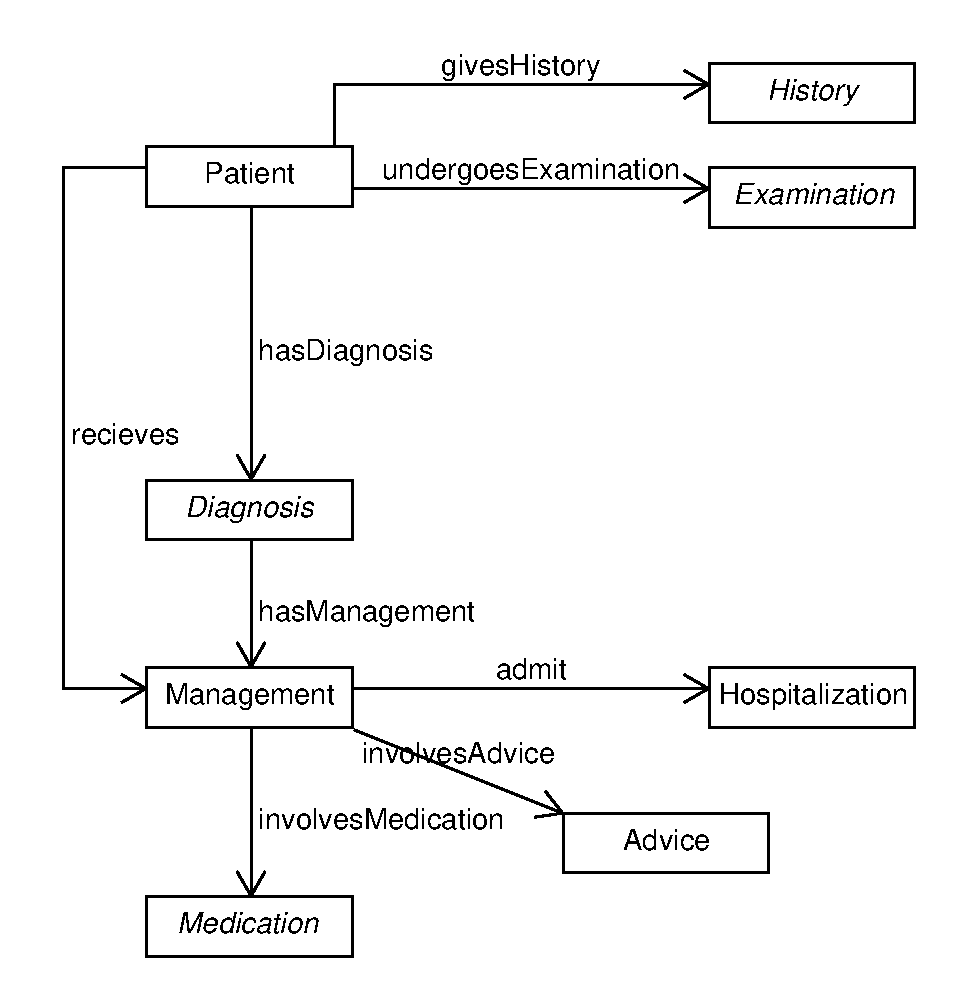
\includegraphics[scale=0.6]{PneumoniaEntityExcerpt}
	\caption {Only an inheritance on the Diagnosis vertex makes the excerpt of pneumonia guideline \parencite{RepublicofKeny2016} different from the original excerpt in figure \ref{fig:EntityGraphExcerpt}}
	\label{fig:PneumoniaEntityGraphExcerpt}
\end{figure}

We see that both pneumonia and possible asthma guidelines have a history part, figure \ref{fig:PneumoniaEntityGraphHistory}, where the patient or dependants can tell something about the condition of the patient. Both guidelines also have an examination part, figure \ref{fig:PneumoniaEntityGraphExamination} where the clinician looks for several symptoms. The symptoms are a bit different from paediatric possible asthma guideline, but they both have several symptoms in common. Wheeze is something the clinician has to be aware about. If the patient is wheezing, the patient should be treated according to the paediatric possible asthma guideline instead.

\begin{figure}[h!]
	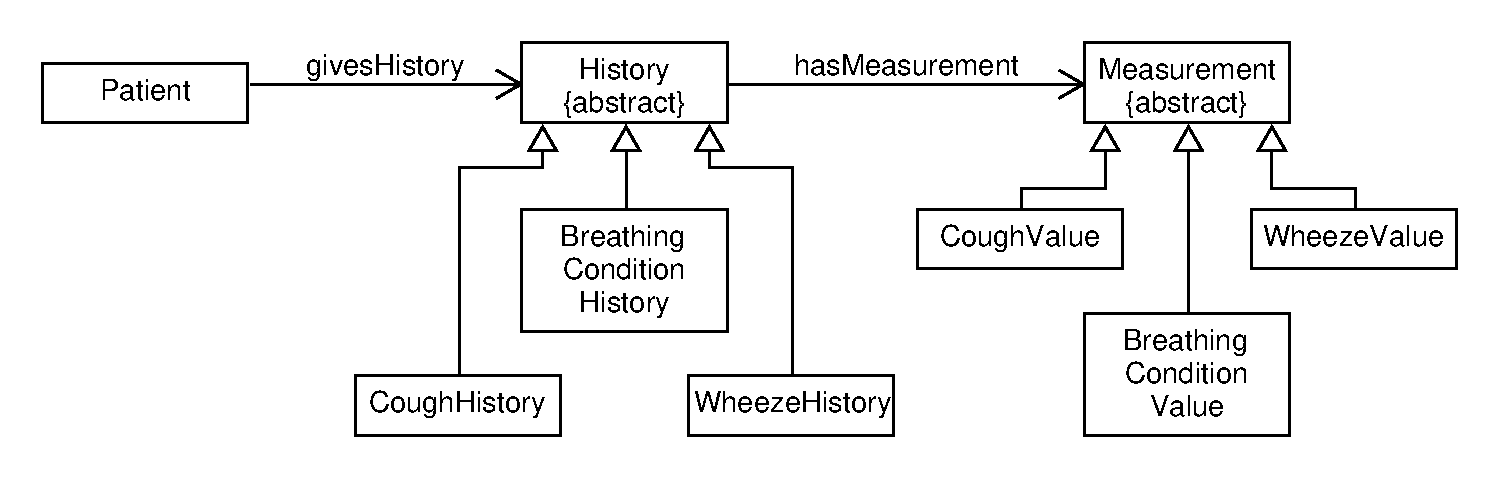
\includegraphics[scale=0.5]{EntityGraphHistory}
	\caption {The history part of the entity model of paediatric pneumonia guideline \parencite{RepublicofKeny2016} is identical to figure \ref{fig:EntityGraphHistory}}
	\label{fig:PneumoniaEntityGraphHistory}
\end{figure}

\begin{figure}[h!]
	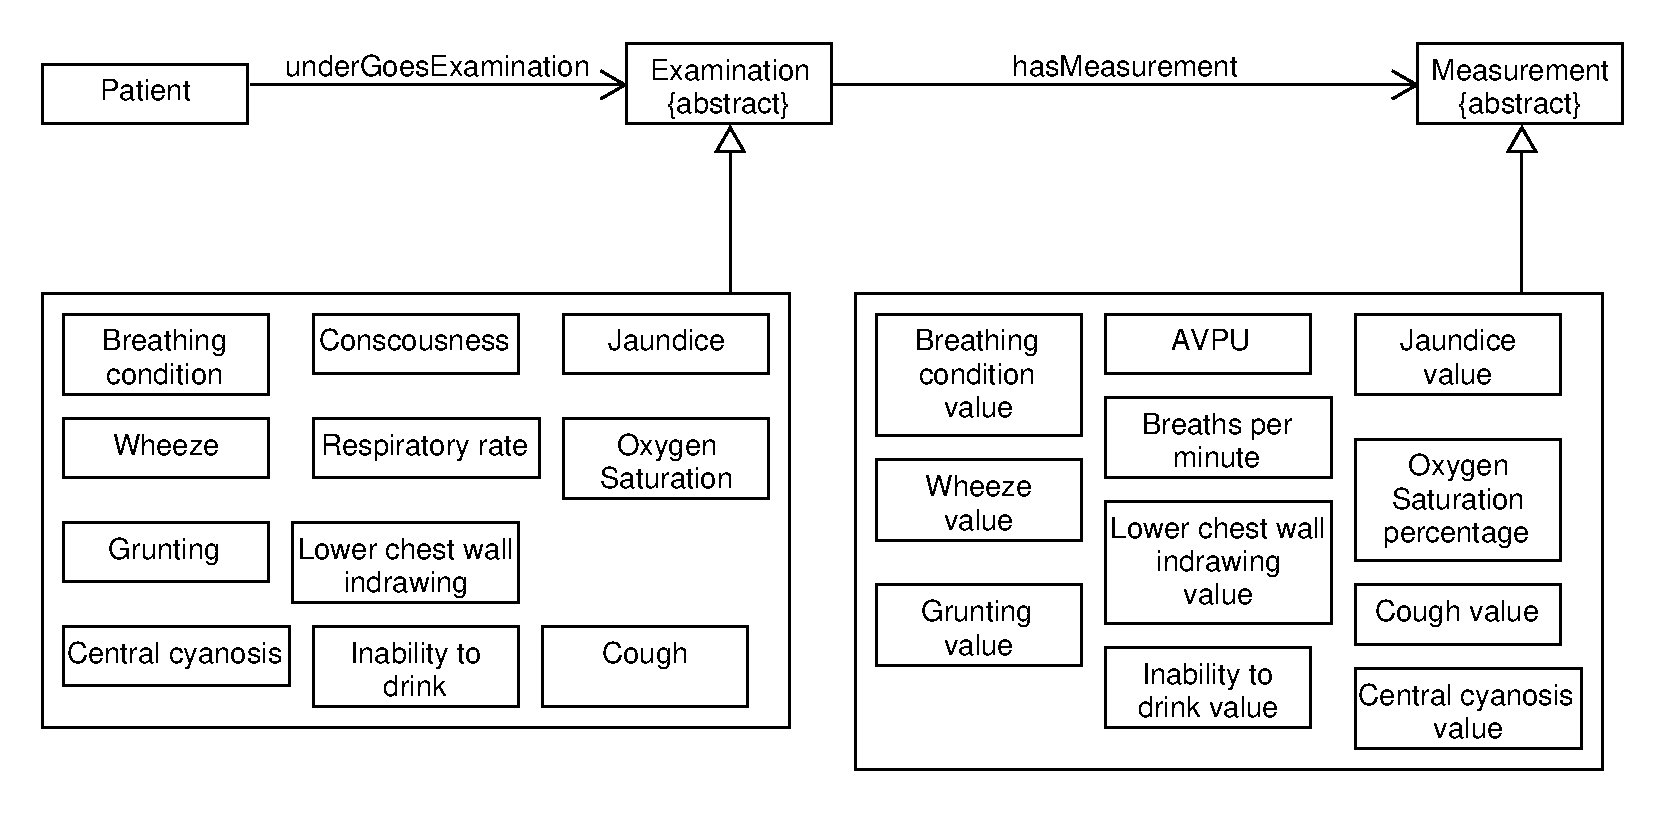
\includegraphics[scale=0.4]{PneumoniaEntityGraphExamination}
	\caption {The symptoms need to be adapted to the paediatric pneumonia guideline \parencite{RepublicofKeny2016} when modelling the examination}
	\label{fig:PneumoniaEntityGraphExamination}
\end{figure}

The big difference is the diagnostic part, figure \ref{fig:PneumoniaEntityGraphDiagnosis}. For the paediatric possible asthma guideline \parencite{RepublicofKeny2016}, there is only one medical condition described. However, for the paediatric pneumonia guideline \parencite{RepublicofKeny2016} patients with tuberculosis or HIV will receive a different treatment. We have not modelled the treatment for pneumonia patients with HIV or tuberculosis as they are separate guidelines. But we need to identify such patients and refer to their respective guidelines. The same goes for asthma. Wheezing patients needs to be identified for asthma treatment.

To support several conditions, we have used inheritance on the diagnosis vertex. A new problem occurs as how should we model tuberculosis, no tuberculosis and that we don't know if the patient has tuberculosis? Earlier on, we used the open world principle for the symptoms. If the vertex doesn't exist, we haven't done the examination for the symptom and we don't know if the patient has it or not. The same goes for diagnosis. If the vertex is not there, we need to clarify if the patient has tuberculosis. To model the situation where we know that the patient hasn't tuberculosis, we have introduced the diagnosis "no tuberculosis". An alternative solution could be to introduce an attribute "status". The attribute could hold information about the patient evidently has the condition, evidently don't have the condition and if it is not clarified. A fourth status could be if the condition is recurring.


\begin{figure}[h!]
	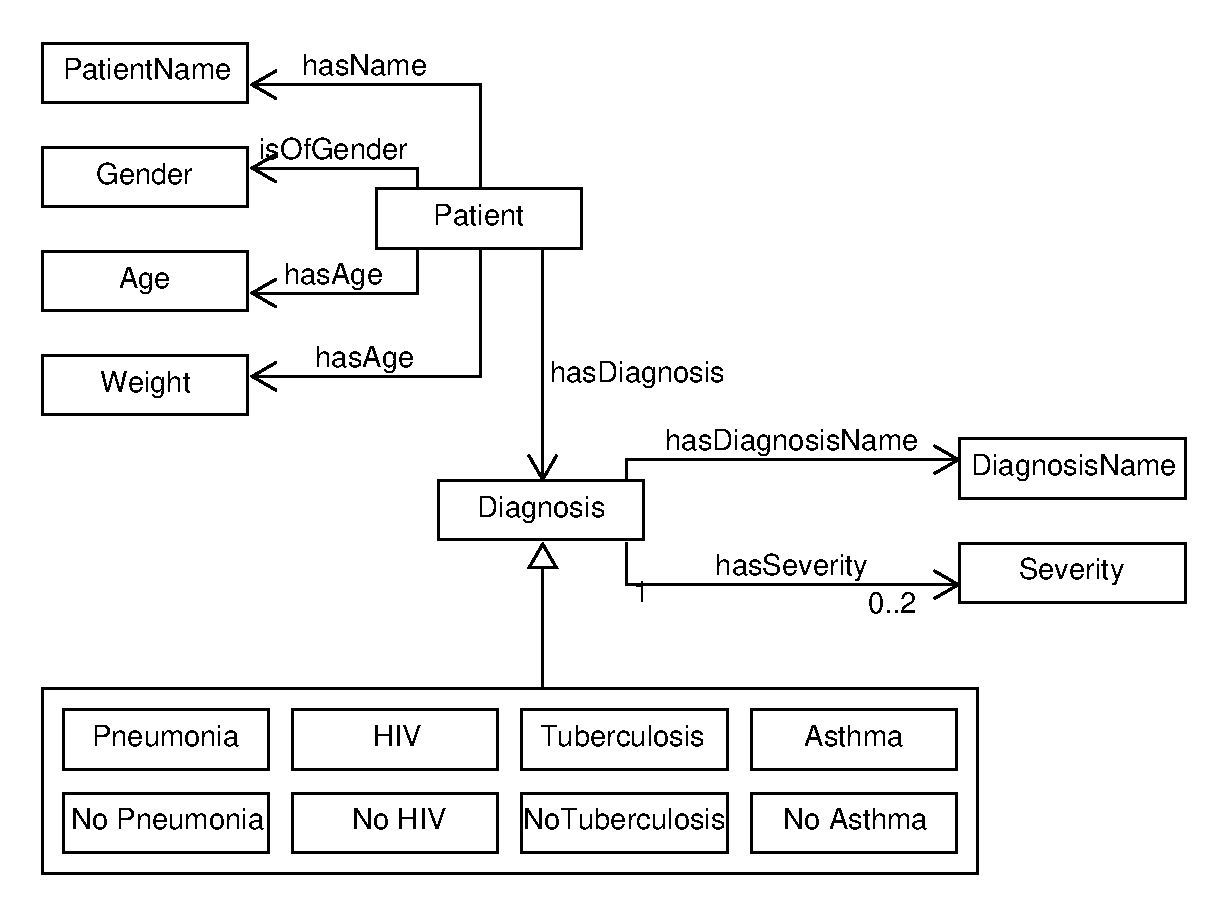
\includegraphics[scale=0.6]{PneumoniaEntityGraphDiagnosis}
	\caption {When modelling the Diagnosis of the paediatric pneumonia guideline \parencite{RepublicofKeny2016}, we need to use inheritance to support differential diagnoses and different treatments when the patient has combinations of diagnoses}
	\label{fig:PneumoniaEntityGraphDiagnosis}
\end{figure}


The management part is also quite similar to the paediatric possible asthma guideline \parencite{RepublicofKeny2016}. The patient and dependants will be given some advise concerning the medical condition of the patient. If the pneumonia is severe, or the patient has lower chest wall indrawing and the patient cannot be reviewed within 48 hours, the patient should be admitted into the hospital. The medication, figure \ref{fig:PneumoniaEntityMedication}, is quite similar to the paediatric possible asthma guideline. For pneumonia there are fewer medications, but both guidelines have treatment with antibiotics and oxygen.

\begin{figure}[h!]
	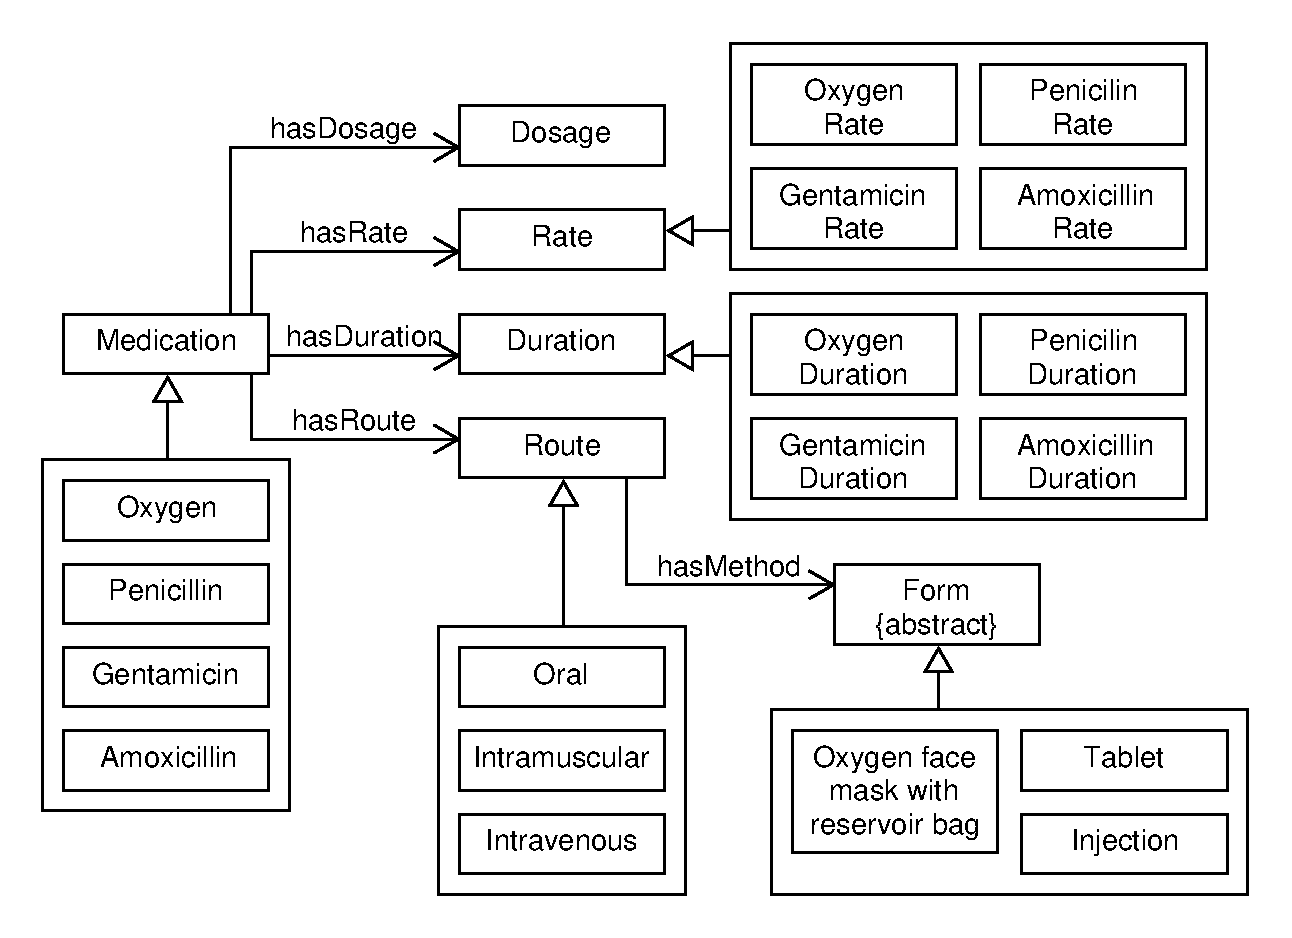
\includegraphics[scale=0.5]{PneumoniaEntityGraphMedication}
	\caption {The paediatric pneumonia guideline \parencite{RepublicofKeny2016} uses oxygen and antibiotic treatment, which can be modelled in the same way as figure \ref{fig:EntityGraphMedication}}
	\label{fig:PneumoniaEntityMedication}
\end{figure}





%\begin{figure}[h!]
%	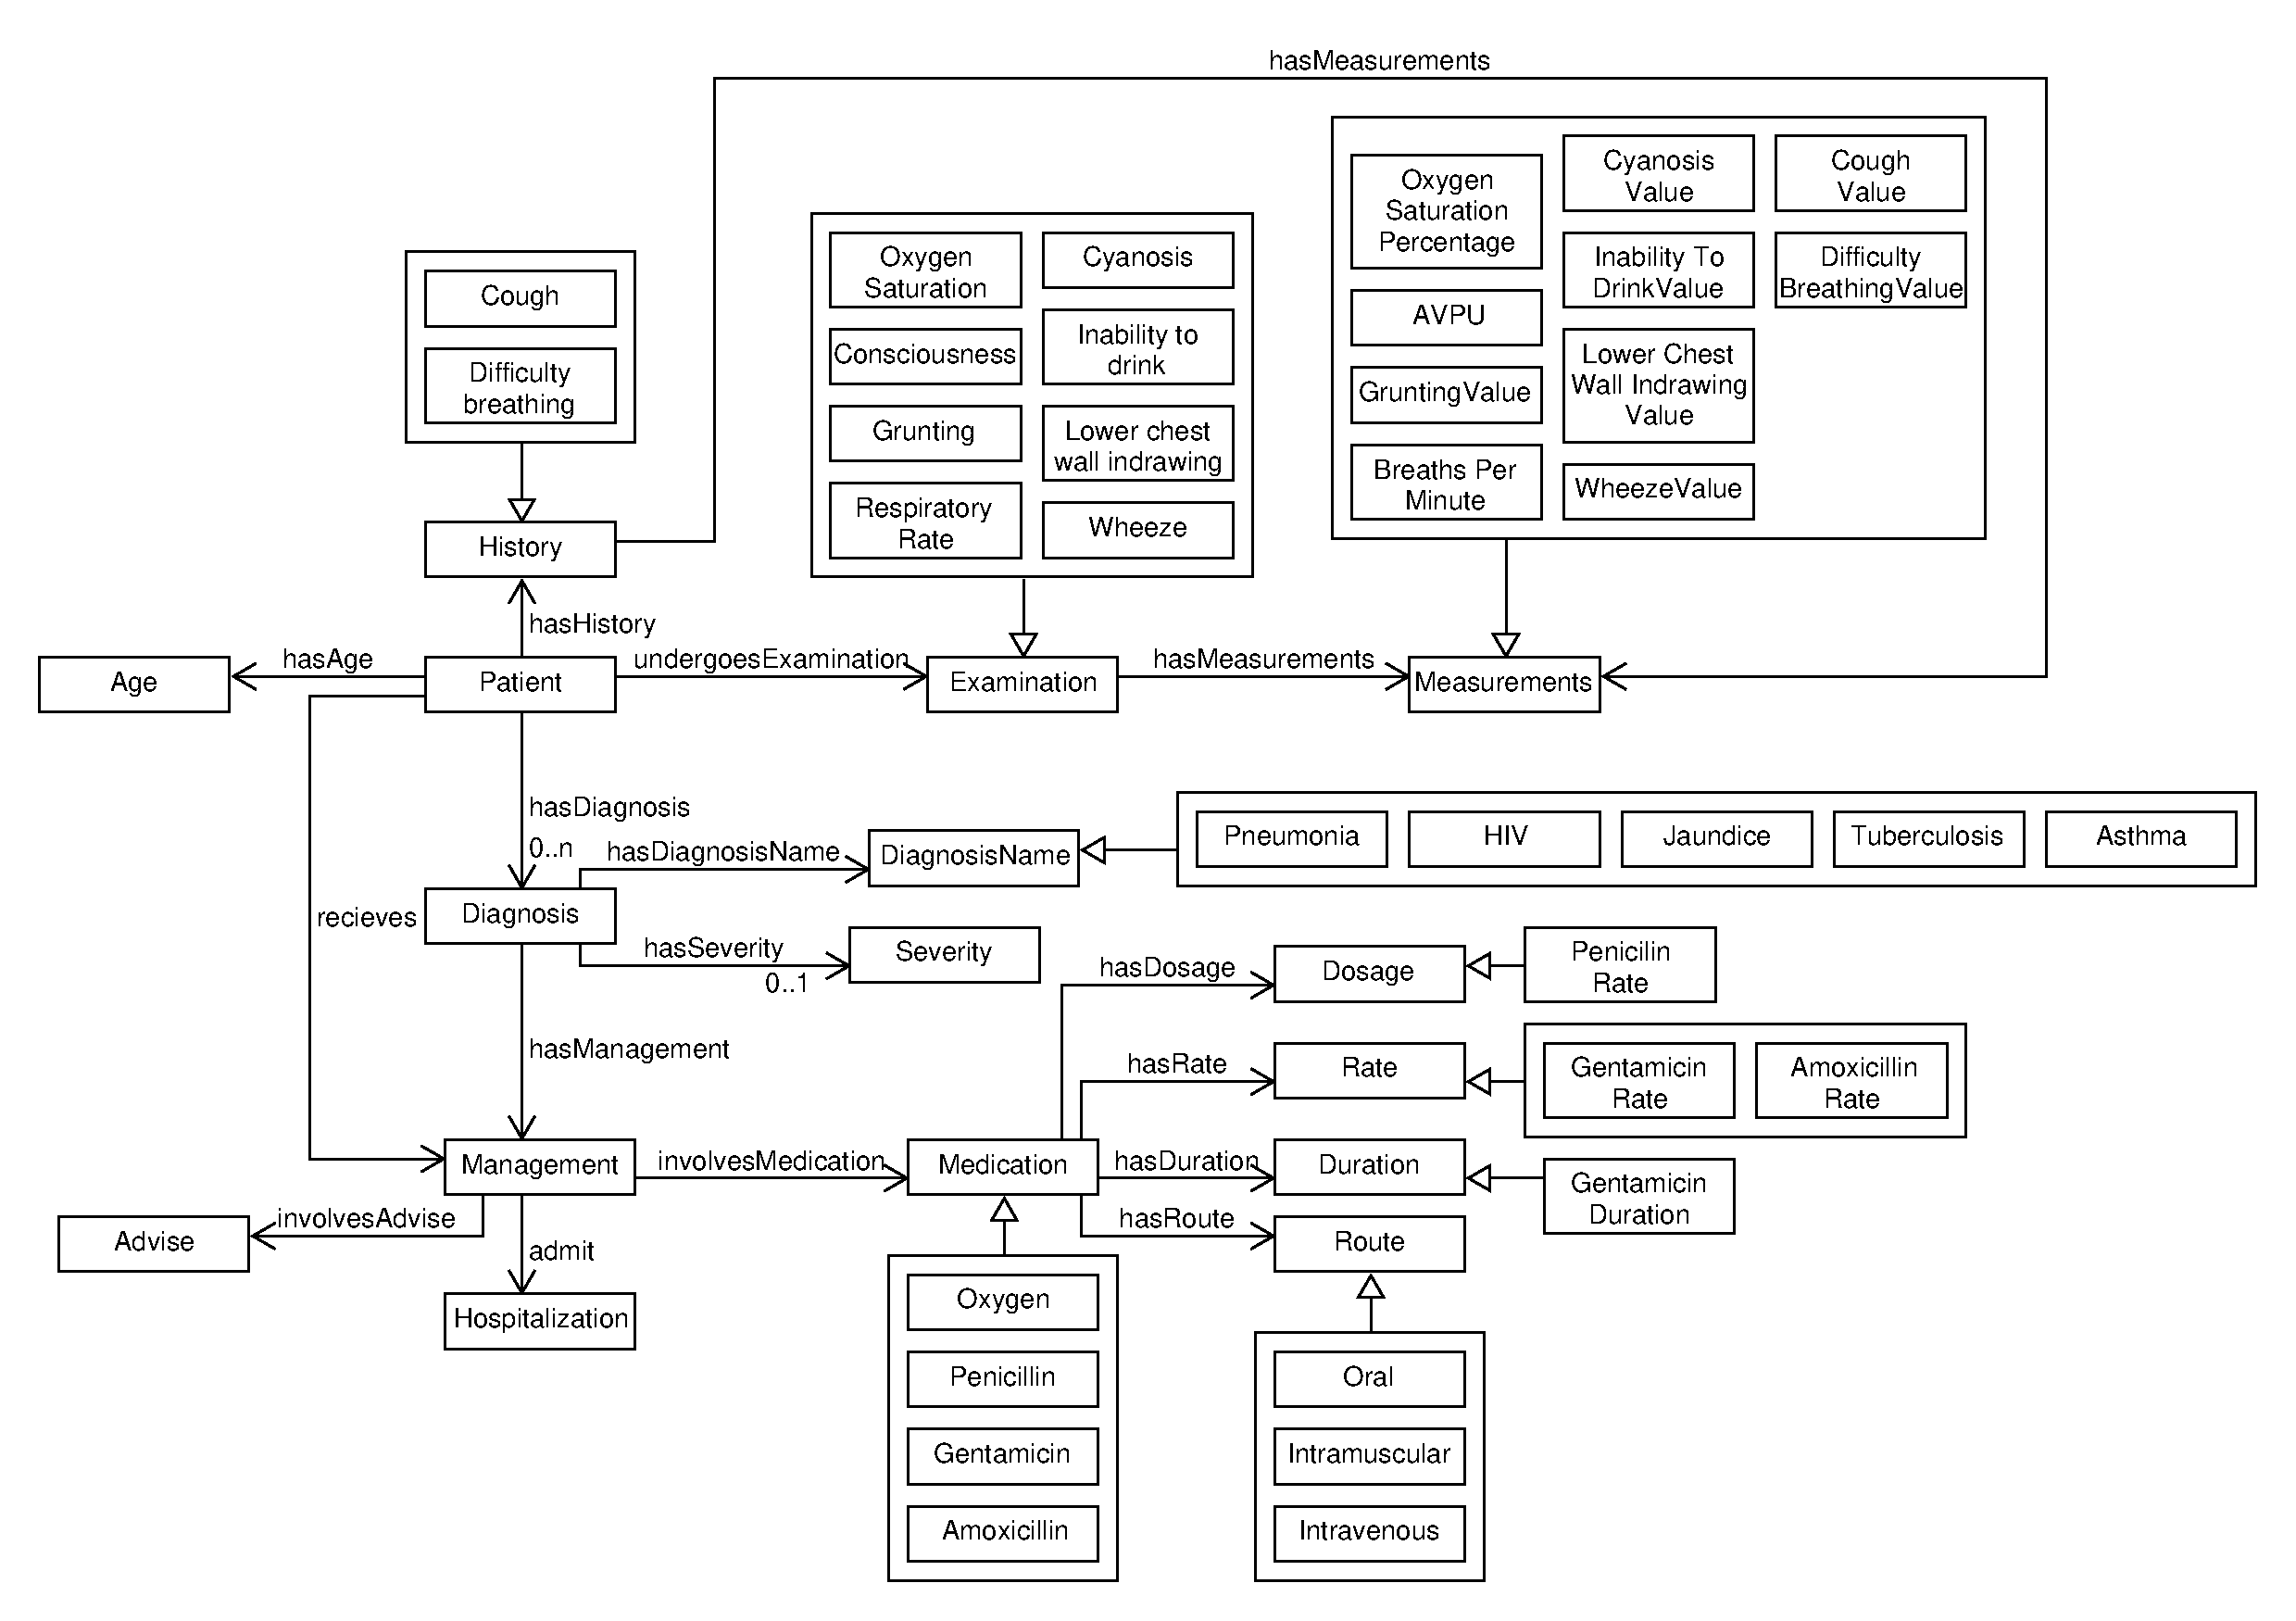
\includegraphics[scale=0.33]{PneumoniaEntityGraph}
%	\caption {We are showing that our model is general enough to represent other CPGs. Here we have modelled the paediatric pneumonia guideline \parencite{RepublicofKeny2016}}
%	\label{fig:PneumoniaEntityGraph}
%\end{figure}

To evaluate the workflow model in figure \ref{fig:WorkflowGraph}, we do like we did for the paediatric possible asthma guideline \parencite{RepublicofKeny2016}. We see the guideline in combination with the entity entity and the workflow model. The paediatric possible asthma guideline \parencite{RepublicofKeny2016} has an assessment part, where we look for patient older than 60 days, cough or difficulty breathing. If he has those symptoms and does not wheeze, we continue looking for other pneumonia symptoms. In the diagnostic part we strengthen our assumption of pneumonia, we set the severity of the diagnosis and we further keep in mind that if the the patient is wheezing he should be given the asthma treatment. Pneumonia patients with HIV or tuberculosis should be referred to specific guidelines for those condition combinations \parencite{RepublicofKeny2016}. In the management part, some patients get admitted into the hospital. The management further has an advise for review within 48 hours. The patients condition is then evaluated either on the hospital for admitted patients, or in a review within 48 hours for other patients. We can conclude with that the workflow model  also covers the paediatric pneumonia guideline \parencite{RepublicofKeny2016}.

In figure \ref{fig:PneumoniaPneumoniaIntegratedEntityWorkflowModels} we demonstrate an instance of the entity model working together with an instance of the workflow model. The patient goes through assessment, diagnosis, management and evaluation. As the patient has jaundice, he won't receive penicillin treatment. As the the pneumonia is severe, the treatment will be evaluated at the hospital and schedule for review is unnecessary. 

\begin{figure}[h!]
	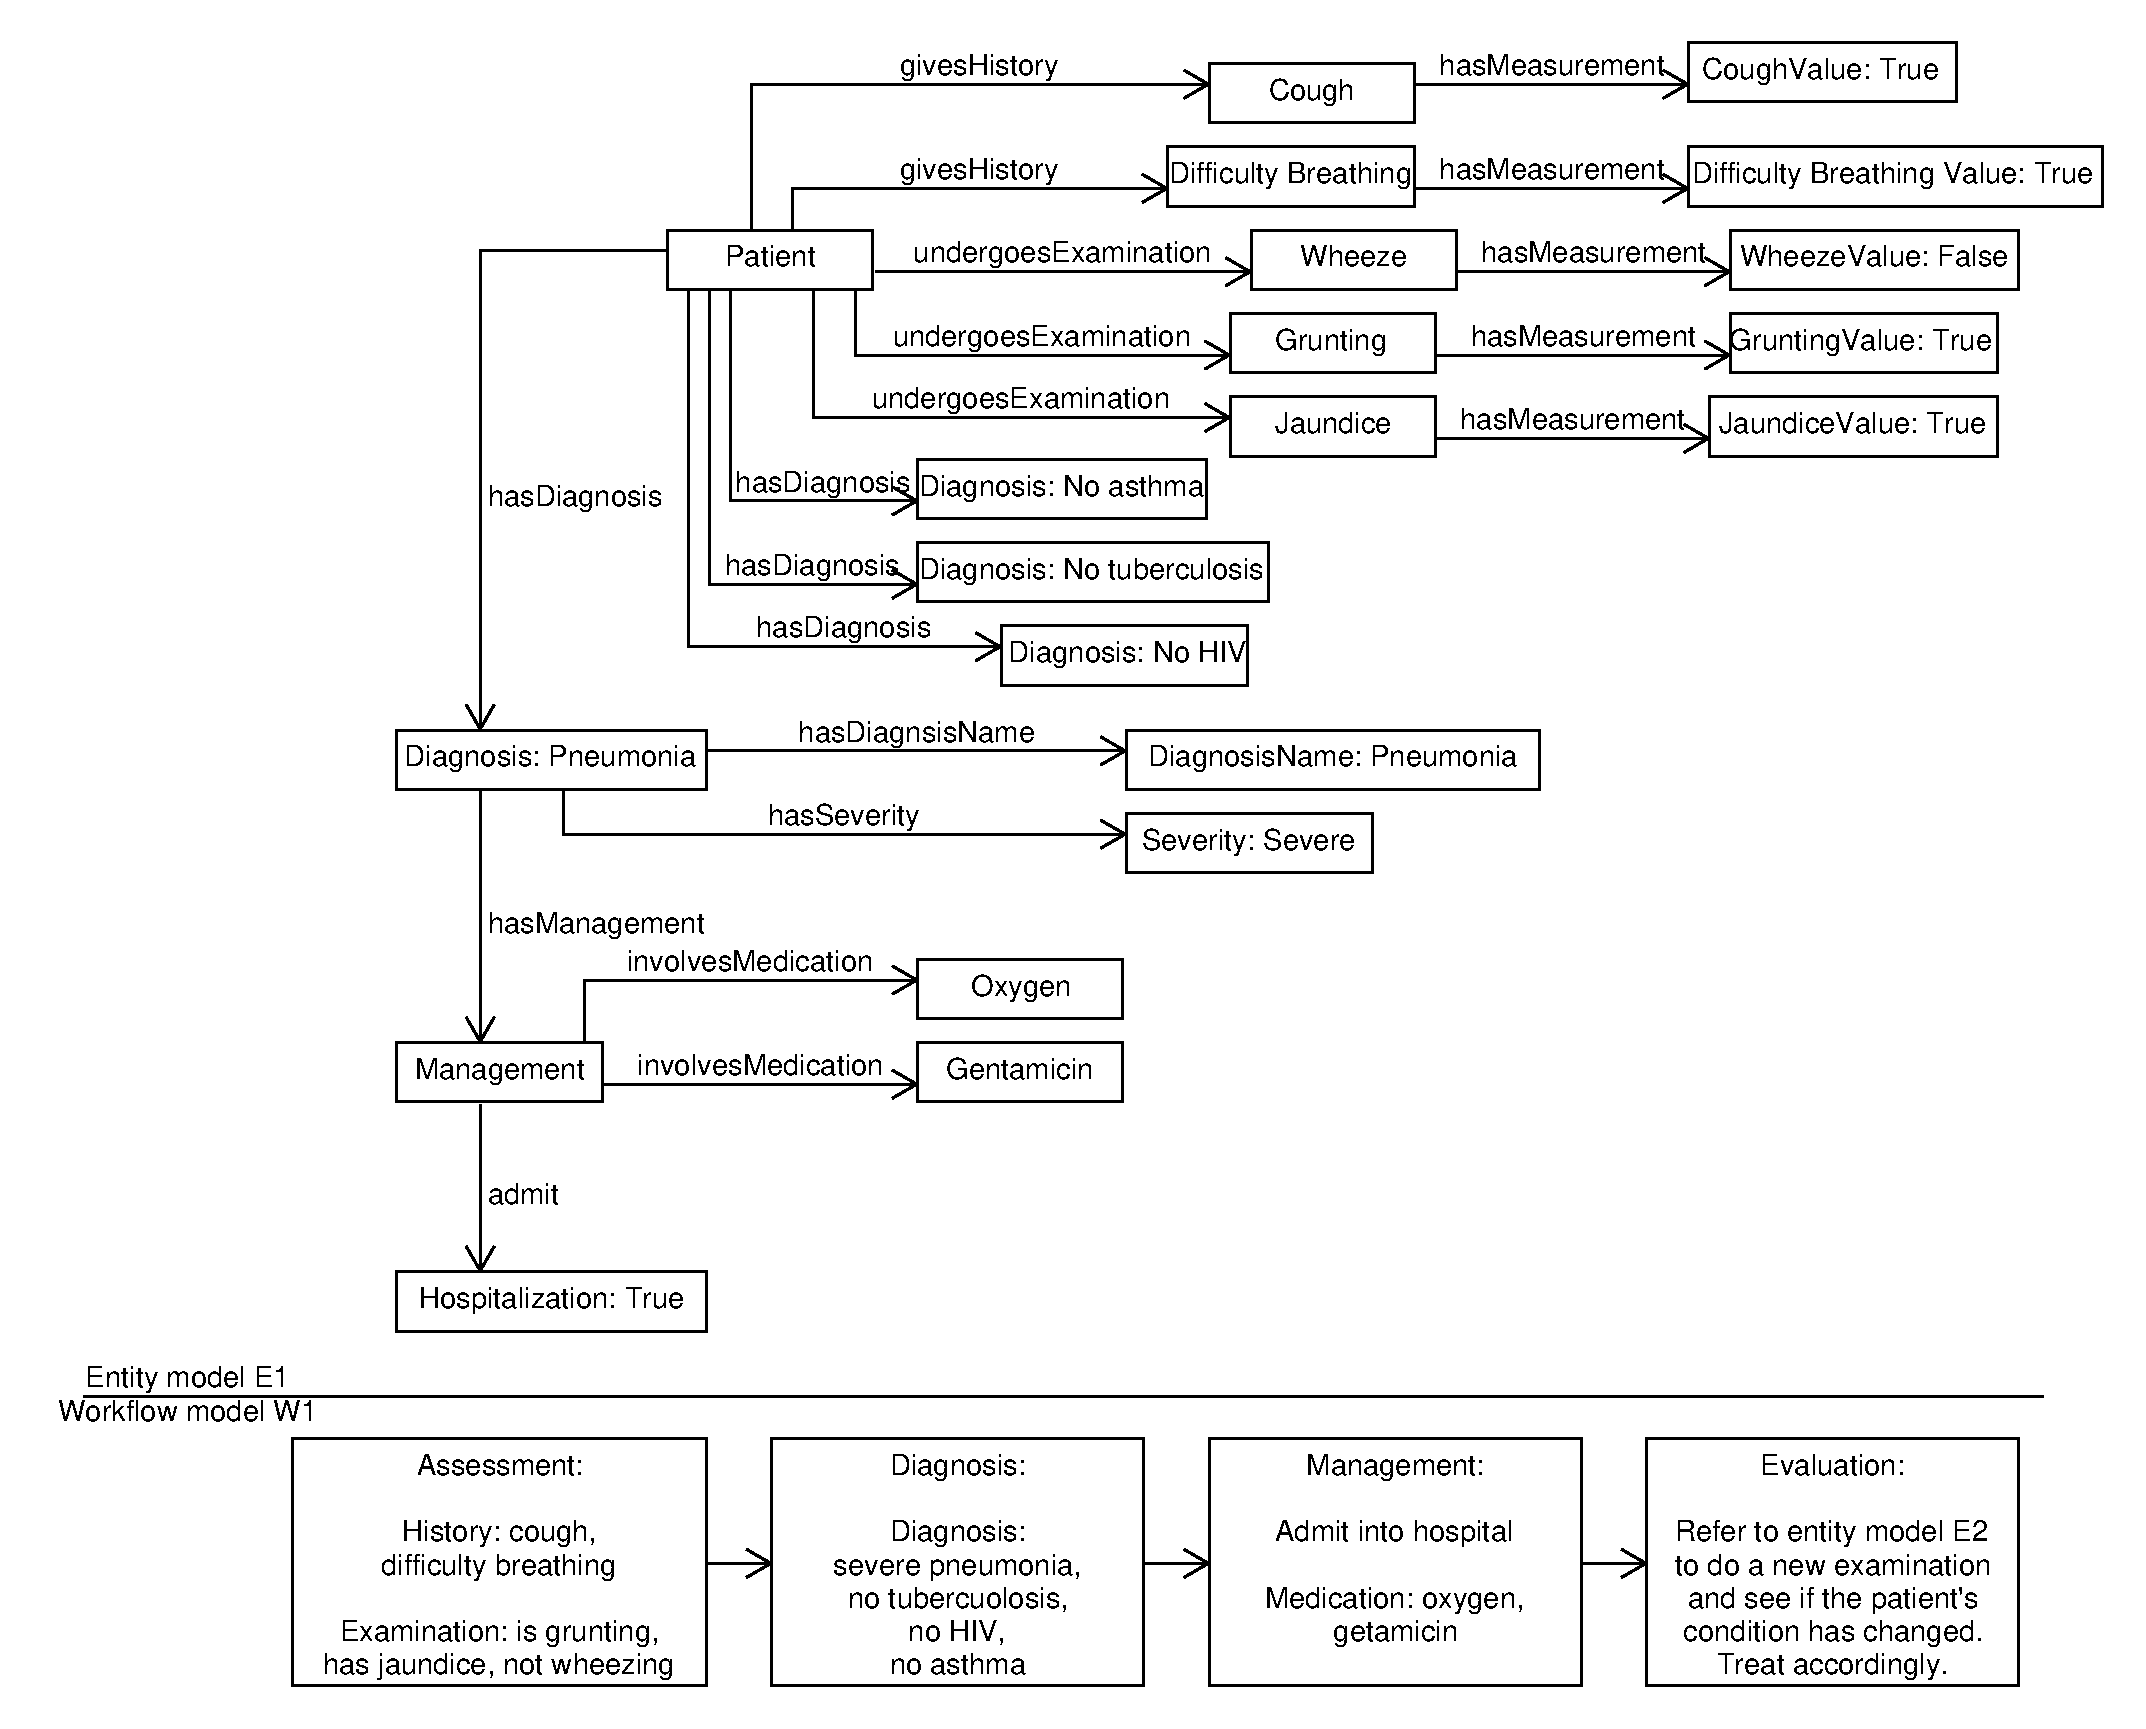
\includegraphics[scale=0.37]{PneumoniaIntegratedEntityWorkflowModels}
	\caption {We are showing out entity model working together with the workflow model for paediatric pneumonia guideline \parencite{RepublicofKeny2016}}	
	\label{fig:PneumoniaPneumoniaIntegratedEntityWorkflowModels}
\end{figure}

After the evaluation, we see that we have modified the entity and workflow models to support both pneumonia and asthma in paediatric medicine. It is likely that further modification and expansion of the entity model is needed when modelling other CPGs. However, we see that we have identified reusable elements of the guidelines, and our models can work as a stepping stone for guideline formalization standardisation.


\subsection{Evaluation of the application}
The evaluation of the application was done with clinicians.	Two medical doctors and two specialist nurses. Both of the specialist nurses are employees at the polyclinic for pulmonary diseases at Haukeland University. One of the nurses is a specialist in sleep apnea, and his master thesis was writing clinical guidelines for sleep apnea. The other nurse is a specialist in asthma, but in adult medicine. The two doctors are educated as general practitioner, but are now working in research.

The evaluation methods were a combination of the cognitive walkthrough and usability test in controlled environment, with follow-up questions. In detail what we did was, the nurses would be asked to play the most difficult level of the game, speak what they are thinking when playing the game and manoeuvring in the application.  The two medical doctors would play the entire game, from the easiest level and to completing the most difficult one. By playing all the levels, the doctors would to far greater extent evaluate the learning model.

Topics to discuss would occur when the clinicians had to think out loud. The master student would observe and take notes when problems and confusions occurred, or that the clinician expressed emotions such as joy, excitement or disappointment. After the clinicians had played through the game, the master student would go through a check-list of topics to discuss. The discussions would be in a semi-structured format, where the check-list worked as a guide. The discussion with the two nurses would be individually, while  the discussion with the two doctors was done in a small focus group, consisting of the two medical doctors and the master student. 

\begin{enumerate}
	\item Can the application be a useful learning tool for medical students, nurses and doctors?
	\begin{itemize}
		\item \textbf{Nurse1:} Very useful indeed. Would be nice to take a test after a lecture about asthma or after having read about asthma to see how much I have learnt and remember. A quiz is far more fun than a check list in paper format. The application is also good for scalability, as you can train a lot of clinicians without adding any resources. Also great if a course leader can see the progress or the level of his students. 
		\item \textbf{Nurse2:} Absolutely useful, and I feel I have learnt a lot by just doing this quiz. The nurse found the game to be very engaging, cheering when getting a correct answer. 
		\item \textbf{Doctors:} For medical doctors, the quiz will be too basic. For nurse it might be good. For medical students it will be very good, as it fits with how the students works and how they will be tested for exams.
	\end{itemize}
	\item How is the flow of the questions? Is the idea of scenarios where we go from assessment, diagnosis, management and follow-up a good approach?
	\begin{itemize}
		\item \textbf{Nurse1:} Happy with the float and the use of scenarios.
		\item \textbf{Nurse2:} Very happy with the float, being able to follow the patient from the start to the end of the treatment.
		\item \textbf{Doctors:} The categories weren't very clear. The questions are floating into each other. One suggestion is to have oxygen and antibiotic administration as own categories. Then you can measure how well they perform in these categories and ask them to repeat the basics if they perform poorly.
	\end{itemize}
	\item Did we manage to present the important elements of the asthma guideline?
	\begin{itemize}
		\item None of the clinicians know the paediatric possible asthma guideline \parencite{RepublicofKeny2016} well enough to answer that question.
		\item {Doctors:} in Norway they usually look at even more parameter. Does the patient smoke? Does he have allergies? The use of CRP to measure the inflammation levels in the body, are just some of the parameters a clinician in Norway would look at.
	\end{itemize}
	\item Is the detail level the element to adjust for the difficulties of questions?
	\begin{itemize}
		\item \textbf{Nurse1:} Yes, but would like to have an even harder level with more details.
		\item \textbf{Nurse2:} Yes, it seems like a right approach. The target group of users is relevant here, that this is meant for the emergency clinic.
		\item {Doctors:} Yes, but the detail level of the questions need to be much harder. One example of going to higher detail level could be "what oxygen administration device would you initially use to a neonate?" to "administering oxygen using nasal prong to a neonate doesn't work. What do you do?". 
		
		In Norway, the patients will visit the hospital with a lot more variation of illnesses and with a higher frequency of less severe diagnoses. Then differential diagnoses gets more important and to represent a lot more clinical conditions as quizzes. The clinicians also work a bit different in Norway. If a patient comes into the hospital with symptoms of severe asthma, they will usually just treat and stabilize the really alarming symptoms and not go through a whole list of treatments.
	\end{itemize}
	\item How are the answer key explanations?
	\begin{itemize}
		\item 
		\item \textbf{Nurse2:} I like how the measurements corresponds and are calculated with the scenario and the patient they are presented with. The answer key explanations gives relevant answers to the questions asked.
		\item \textbf{Doctors:} The answer key explanations are good. We like that we get an explanation when we answer correctly. We preferred to try until getting the answer correctly rather than clicking "learn more" and proceed to next question. It could be nice to get an explanation why the answer was wrong, but we are rather impatient, we want to proceed and find the correct answer quickly.
	\end{itemize}
\end{enumerate}

The quality of game questions:
\begin{enumerate}
	\item The assessment, none of the distractions is a wrong answer. Even though wheeze is what we are looking for.
	\item When asking for salbutamol dosage, it is relevant to know where and in which stage of the treatment it is being given. Also saying something about rate or duration can help clarify that.
	\item Very nice that we in some questions change the way we ask. Sometimes we give a diagnosis and asks which symptoms identifies it. Then we give some symptoms and then ask about the diagnosis.
	\item In the assessment part of the scenarios, we tell that clinical encounter happens at the emergency clinic. But we should find a way to amplify it even more, as one of the test persons missed that detail.
	\item Descriptions such as "age > 12 months" is hard for clinicians to read. We should avoid using logical operands.
	\item "Recurrence of asthma" is unclear. Who says that it is recurrent? Is it recurrent when the patient is in the emergency clinic? Does the patient tell that it is recurrent? Is it in the journal? All the clinicians had commented on the use of recurrence.
	\item We have a trick question and we should avoid those. We ask what is not the right way to administer salbutamol to a patient. The answer is oral. The clinician thought the right answer could be one of the other alternatives as an oral version of salbutamol doesn't exist.
	\item We are using history i an imprecise way. History is not only what the patient or the caregiver tells. The patient can have been visited the hospital for that symptom earlier or have had it in an earlier point of time. It may be something from their journal. More detail where and when the history comes from is needed. 
\end{enumerate}

User interface and game experience
 \begin{enumerate}
 	\item All the clinicians were very positive to the multiple-try with hint approach. When they give a wrong answer, they get a new chance to revise the question and correct their answer.
 	\item When the clinicians answer a question incorrectly, they are presented with a "learn more" button. When they click on this button they get presented with an answer key explanation. When they click on "next" the nurses get very surprised and disappointed that were taken to the next question and don't get the chance to get the question right. The medical doctors were fine with that approach.
 	
 	Here the specialist in asthma had a very interesting suggestion. When she clicks on "learn more", she want an explanation of why that suggestion was wrong or in which situations that answer would have been correct. Then she want to try again to collect the reward. She was noticeably disappointed at the summary when she saw that she was penalized hard for clicking "learn more".
 	\item The clinicians wanted a link or a button to display the clinical guidelines in the screen they were presented with the answer key explanation. Then they can read and learn more.
 	\item The clinicians noticed that they didn't have to remember details from the previous question before they answered the next. That was something they appreciated.
 	\item The two doctors didn't think text questions were the best approach. They wanted pictures, sound and perhaps short film clips, and the text could come as a supplement. A picture with a blue face just lying in the bed, would be a severe case of asthma indeed, by just observing the picture. A child sitting and playing while having difficulty breathing could be a case of mild or moderate asthma. A sound clip of an asthma patient wheezing or the gurgling sound of a breathing pneumonia patient could also be helpful. A patient sitting in the bed, getting oxygen through the nose, would say something about the treatment given and the evaluation of the patient. Perhaps a film clip where the clinician tries to talk to the patient. The use of film, pictures and sound would provide more realistic scenarios to what the clinicians will meet at the hospital.
 	\item When having met the passing condition of one of assessment, diagnosis, management and follow-up, it is a good thing that the passed category gets excluded from the quiz when replaying the level. This makes the game less tedious.
 	\item In the situation where the user performs very poorly and gets demoted from a difficulty level, an explanation should be shown.
 	\item The two doctors meant the "wrong" hint in red when answered a question incorrectly was ok. If sugar coating the feedback, the satisfaction of getting a green "correct" would have been dampened.
\end{enumerate}





\subsection{Results}
Here we make a brief summary of the results from the evaluation. We want to verify that we have data models at an abstraction level such that they can be used to represent other clinical practice guidelines. The models will be our contribution to the science of health informatics. We want to ensure that our serious game is a valuable contribution to the medical community. Contribution to science and to the community are requirements from design science.

\paragraph{Evaluation of the models}
We have shown by a practical example how the entity model can be used to represent the paediatric guideline of pneumonia \parencite{RepublicofKeny2016}. A requirement was identified and met by making an abstraction of the Diagnosis in the entity model. This was necessary to support differential diagnosis, and to support treatments which are dependent on which other diagnoses the patient may have. 

We showed how we could make instantiations of the entity and workflow models and how they work together to represent a full clinical encounter for patient suffering from pneumonia.


\paragraph{Evaluation of the application}
In table \ref{table:AppEvaluation}, we have made a brief summary, where we quantify the evaluation of the game application. The  
\begin{table}[h!]
	\begin{tabular}{ | m{18em} | m{4em}| m{4em} | } 
		\hline
		\textbf{Questions} & \textbf{Positives} & \textbf{Negatives}\\
		\hline
		\textbf{Can the game be a useful learning tool for} &  &  \\
		Medical students? & 2 & 0 \\
		Nurses? & 2 & 0 \\
		Doctors & & 2 \\
		\hline
		\textbf{How is the flow of the questions in scenarios} & 2 & 2 \\
		\hline
		\textbf{Is adjusting the detail level to make questions more difficulties the right approach?} & 4 & 0 \\
		\hline
		\textbf{Is the quality and approach answer key explanations correct?} & 3 & \\
		\hline
		\textbf{Number of feedbacks about the quality of quiz questions} & 1 & 7 \\
		\textbf{User experience} & & \\
		Wants the possibility to read the guideline in the game & 4 & 0  \\
		Didn't have to remember details from previous screen & 3 & 0 \\
		Textual questions instead of multimedia & & 2 \\
		\hline
		\textbf{Game elements} & & \\
		Multiple-try feedback & 4 & 0 \\
		"Learn more" doesn't give a last attempt to get the question right & 2 & 2 \\
		\hline
		\textbf{Learning model} & 2 & 0 \\
		Don't repeat questions from completed quiz categories & 2 & \\
		\hline
	\end{tabular}
	\caption{}
	\label{table:AppEvaluation}
\end{table}

\section{Findings}
Here we will relate our findings to the research questions.

\paragraph{\textbf{RQ1:} Based on clinical guidelines, how can we define and represent a generic data structure that can be used to implement applications such as online guidelines or training games for such guidelines, and where applications can adapt to the level of their users?}

For this research question, we have proposed four data models. The first two data models are a domain (entity) model \ref{fig:GeneralEntityGraph} and a guideline (workflow) model \ref{fig:WorkflowGraph}. The domain model represents a patient, his symptoms, medical condition and what the clinicians do to mange his medical condition. The guideline model represents the steps in a clinical encounter. When the domain model and the guideline model work together, we can represent the patient, symptoms, diagnosis and management of the medical condition for every step through the clinical encounter. The model allows us to make online guidelines or training games with specific patients examples through the whole guideline.

We also proposed a student learning model and a game model. By using Dynamic Content Management \parencite{Eide2008}, we showed how we can split the learning content into content units. Each of these content units contain learning resources and evaluations at different difficulty levels. In that sense, the learning content can be adapted to knowledge of the student. Presenting difficult evaluations in areas where the student is strong, and easier evaluations where the student is weak. 

\paragraph{RQ2: Can the generic data structure in RQ1 be used to generate a specific data model for another domain such as paediatric asthma?}

In figure \ref{fig:EntityGraphExcerpt}, \ref{fig:EntityGraphHistory}, \ref{fig:EntityGraphExamination}, \ref{fig:EntityGraphPatientDiagnosis} and \ref{fig:EntityGraphMedication}, we showed a specific entity model for the paediatric guideline of possible asthma \parencite{RepublicofKeny2016}. 

In figure \ref{fig:IntegratedEntityWorkflowModels}, we show an instantiation of the specific entity model, working together with an instantiation of the workflow model. This shows that also the workflow model can be used for a specific domain.

For the student learning model, game model, entity model and workflow model, we also did a proof of concept. We developed a serious game which tested students in the paediatric guideline of possible asthma \parencite{RepublicofKeny2016}. Then the student learning model and the game model got applied for a specific domain, in this case paediatric possible asthma.

\paragraph{RQ3: How can we use the data model in RQ2 to implement a game for guideline training that can adapt to the level and progression of users?}

For the student learning model and the game model, we have applied the Dynamic Content Management \parencite{Eide2008}. We have split the learning content into content units to be able to adapt the learning content to the knowledge level of the student. Then we identify knowledge dependencies between the content units. When the student progresses, we can provide more difficult questions, given that the knowledge dependencies are followed. This ensures that the student has the basic understanding in relevant subjects to progress.

We make the difficulty level tougher by adding more details to the questions. Going from factual statements, to scenarios to detailed scenarios.

The adaption to the level and progression of users were demonstrated in the serious game.

\paragraph{RQ4: Is the guideline meta model at an abstraction level such that it can be used for other guidelines?}

In figure \ref{fig:PneumoniaEntityGraphExcerpt}, \ref{fig:PneumoniaEntityGraphHistory}, \ref{fig:PneumoniaEntityGraphExamination}, \ref{fig:PneumoniaEntityGraphDiagnosis} and \ref{fig:PneumoniaEntityMedication}, we demonstrate how the entity model can be used to to represent the paediatric guideline of pneumonia \parencite{RepublicofKeny2016}. However, the model modifications to be able to support differential diagnoses and the situation where the treatment depends on which other diagnoses the patient has.

In figure \ref{fig:PneumoniaPneumoniaIntegratedEntityWorkflowModels} we show an instance of the specific entity model working with an instantiation of the workflow model. This shows that the workflow model is at an abstraction level such that it can be used for other guidelines.

The student learning model and game model divides the learning content into content units based on the workflow model. When the workflow model is abstract enough to be used the paediatric guideline of pneumonia \parencite{RepublicofKeny2016}, then the student learning model and the game model would be as well. 



\subsection{Limitations of the entity model}
\begin{itemize}
	\item We can't ask questions like "what are the symptoms for severe asthma?". The entity model is a model of one specific patient at one stage in the clinical encounter. To have severe asthma he may only have one of the symptoms for severe asthma and not all of them.
	\item It is difficult to ask what NOT to do. If the vertex doesn't exist, only an empty string is returned. "NOT to do" can only be used were we actually have specified that the action should not be done. An example is "don't admit to the hospital" where we have specified "no" at the Hospitalization vertex.
	\item The inheritance makes it difficult to generalize some questions. We can't make a template which asks about the Rate a (any) medicine should be taken with. We need to specifically ask for that medicine. To be able to ask for a general medicine, one solution can be to introduce a new tag which compares the substring of the type of the vertex. Another solution is to use the meta model and not the instance model. In future work we can study GraphQL to see if it can be used as another alternative to solve this problem.
\end{itemize}

\section{Summary}
In this chapter, we have evaluated the  entity and workflow models by showing that they can be used to represent other guidelines, such as the paediatric pneumonia guideline \parencite{RepublicofKeny2016}.

We have evaluated the serious game with two nurses and two medical doctors to ensure that we are delivering value to the medical community.

We have discussed the findings in relation to the research questions, and we have identified some of the limitations of the entity model.  
	

